\documentclass[tikz, border=5pt]{standalone}
\usepackage[utf8]{inputenc}
\usepackage[T1]{fontenc}
\usepackage{xcolor}
\usepackage{tikz-3dplot} % Useful for 3D perspectives

% --- Definimos un color rojo oscuro personalizado ---
\definecolor{darkred}{RGB}{140, 21, 21}

\begin{document}

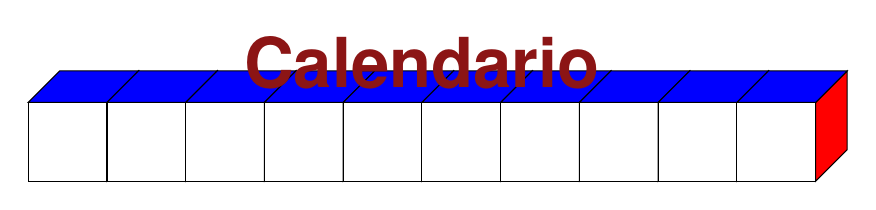
\begin{tikzpicture}
    % -----------------------------------------------------------------
    % OPCIONAL: Fondo negro como en la imagen de ejemplo
    % Para usarlo, descomenta la siguiente línea.
    % \fill[black] (-1,-1) rectangle (11, 3);
    % -----------------------------------------------------------------

    % --- Bucle para dibujar los 10 cubos ---
    % La variable \x va de 0 a 9, dibujando un cubo en cada paso.
    \foreach \x in {0,...,9} {
        % Usamos un 'scope' para aplicar un desplazamiento a cada cubo
        \begin{scope}[shift={(\x,0)}]
            % Dibujamos las 3 caras visibles del cubo
            % Todas tienen borde negro (por defecto) y relleno blanco
            \draw[fill=white] (0,0) rectangle (1,1);                                     % Cara frontal
            \draw[fill=red] (1,0) -- ++(0.4,0.4) -- ++(0,1) -- ++(-0.4,-0.4) -- cycle; % Cara lateral derecha
            \draw[fill=blue] (0,1) -- ++(0.4,0.4) -- ++(1,0) -- ++(-0.4,-0.4) -- cycle; % Cara superior
        \end{scope}
    }

    % --- Texto superpuesto ---
    % Colocamos un nodo en el centro horizontal (x=5) y por encima de los cubos (y=1.7)
    % Usamos una fuente sans-serif (phv), en negrita (\bfseries) y tamaño grande (\Huge)
    \node at (5, 1.5) {\fontfamily{phv}\selectfont\Huge\bfseries\color{darkred}Calendario};

\end{tikzpicture}


\begin{tikzpicture}[tdplot_main_coords] % Use tdplot_main_coords for 3D perspective
    % Define coordinates for the cube's vertices
    \coordinate (A) at (0,0,0);
    \coordinate (B) at (2,0,0);
    \coordinate (C) at (2,2,0);
    \coordinate (D) at (0,2,0);
    \coordinate (E) at (0,0,2);
    \coordinate (F) at (2,0,2);
    \coordinate (G) at (2,2,2);
    \coordinate (H) at (0,2,2);

    % Draw the visible edges
    \draw (A) -- (B) -- (C) -- (D) -- cycle; % Bottom face
    \draw (E) -- (F) -- (G) -- (H) -- cycle; % Top face
    \draw (A) -- (E);
    \draw (B) -- (F);
    \draw (C) -- (G);
    \draw (D) -- (H);

    % Draw the hidden edges (optional, can be dashed)
    % \draw[dashed] (A) -- (D);
    % \draw[dashed] (A) -- (E);
    % \draw[dashed] (D) -- (H);

\end{tikzpicture}
\end{document}